\subsection{Third Research Question}
\label{sec:ResearchQuestion3}
The third research question of this project states:
\\
"How can the model be visualized to enforce explainability?"
\\\\
The proposed SCVM, modelling dynamic networks using velocity dynamics in Euclidean latent space, specifically enables the modelling of an explainable representation.
The results presented in this section seek to evaluate to what extend this explainability is present, and what impact applying rotation correction and regularization has.


\subsubsection{Position Correction}
\label{sec:ResearchQuestion3:PositionCorrection}
The first investigation of explainability deals with the impact of implementing position correction in the SCVM.
The SCVM without any form of correction or regularization will fit its parameters in accordance to the intensities of interactions between nodes.
This means the SCVM is \textit{only} concerned with the reciprocal distances between nodes at given time points.
These inter-node distances are in themselves indifferent to the positions drift of the entire system of nodes.
The animation in the link below shows the SCVM trained for 5000 epochs, fitted with 100 steps to the Resistance real dataset 1, see section\ref{sec:Data:RealData:RealDataset1}, without any position correction at all.

LINK NO POSITION AND DRIFT CORRECTION
\\
\noindent
As can be seen, the animation shows a system of interacting nodes drifting in the latent space.
While the dynamic network of a game of Resistance is represented correctly in the animation, the fact that it is drifting in latent space makes understanding the dynamics of the system less straight forward.
\\
In order to enforce explainability and make it easier to interpret the dynamics of the system correction of positions and drift is applied, as explained under section \ref{sec:Method:ProposedModel:PositionCorrection}.
Training the SCVM with position and drift correction yields the animation in the link below.

LINK POSITION AND DRIFT CORRECTION
\\
\noindent
The above animation shows the exact same dynamics, but in a stable frame of the latent space centered around the coordinates (0,0) without the positional noise, which provides a more intuitive animation.


\subsubsection{Rotation Correction}
\label{sec:ResearchQuestion3:RotationCorrection}
With the correction of positions and drift, the animations are more easily interpretable and serve a better foundation of being able to infer and explain what is going on in the given dynamic network.
As with positions and drift, the rotation of the given system does not impact the inter-node distances, and can hence be neutralized as explained under section \ref{sec:Method:ProposedModel:RotationCorrection}.
An animation of the Resistance game, again trained for 5000 epochs, fitted with 100 steps, is shown in the link below:

LINK ROTATION CORRECTION
\\
\noindent
What this animation entails, while being similar to the one with position and drift correction applied, is a standardized system rotation, in which the most movement happens along the x-axis, regardless of which dynamic network is modelled.




\subsubsection{Regularization}
\label{sec:ResearchQuestion3:Regularization}
In order to further enforce explainability with the visualizations of a given dynamic network, a regularization parameter is added as explained under section \ref{sec:Method:ProposedModel:Regularization}.
\\
The evaluation of the impact from applying various degrees of regularization is based on animations of the SCVM fitted to the Resistance game dataset as with the above results of corrections.
The animation shown in the link below is the SCVM fitted to 100 steps, with correction of positions, drift, and rotation, and trained for 5000 epochs:

RESISTANCE UDEN REGULARISERING
\\
The velocities in latent space for all nodes, while to some extend being regularized by the modelling approach, are free to change drastically between each step.
While the above animation visualizes how the 8 players and computer (P0) interact with each other over the duration of the game, their movements in latent space are to some extend changing drastically, seen by their shootings back and forth through latent space.
In order to change this, with the goal of making inter-step changes less drastic, the model is regularized.
\\\\
The animations of regularization with values $\gamma = [0.1, 0.5, 1.0, 2.5, 5.0, 10.0]$:
\\\\
With regularization $\gamma = 0.1$:
RESISTANCE MED REGULARISERING 0.1
\\\\
With regularization $\gamma = 0.5$:
RESISTANCE MED REGULARISERING 0.5
\\\\
With regularization $\gamma = 1.0$:
RESISTANCE MED REGULARISERING 1.0
\\\\
With regularization $\gamma = 2.5$:
RESISTANCE MED REGULARISERING 2.5
\\\\
With regularization $\gamma = 5.0$:
RESISTANCE MED REGULARISERING 5.0
\\\\
With regularization $\gamma = 10.0$:
RESISTANCE MED REGULARISERING 10.0
\\\\
These animations WRITE ABOUT ANIMATIONS

\subsubsection{Animation Showcase: Lyon Primary School}
\label{sec:ResearchQuestion3:Lyon}

As a final evaluation of the explainability of the SCVM learned dynamics, the Lyon Primary School dataset, see real dataset 2 under section \ref{sec:Data:RealData:RealDataset3}, is fitted.
\\\\
This dataset has labels for all nodes, which tells us which class each pupil belongs to, if not a teacher, and so can be interpreted with some added information.

LYON ANIMATION
\begin{figure}[H]
    \centering
    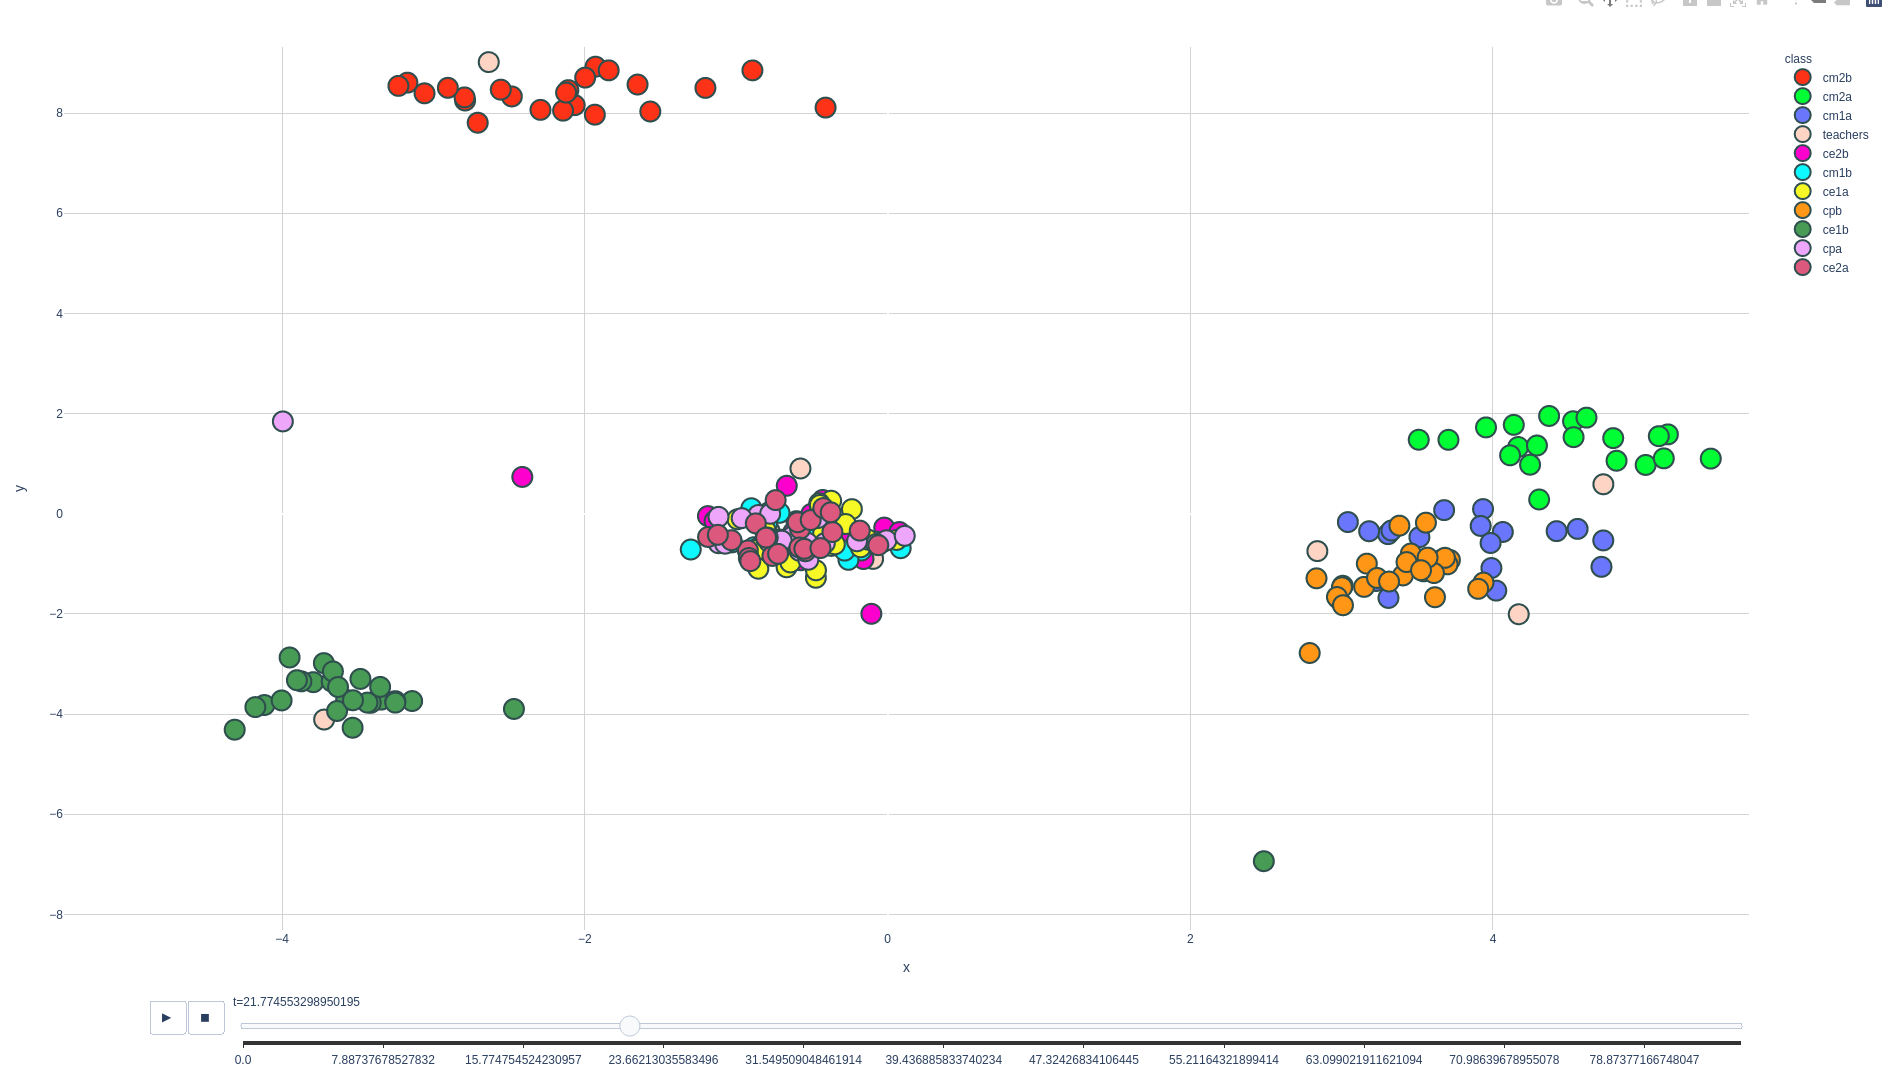
\includegraphics[width=\textwidth]{0_images/lyon_screenshot.png}
    \caption{Screenshot from Lyon Primary School fitted SCVM. Each color represents a different school class of pupils, while the teachers can be see near one class each in some cases.}
    \label{fig:LyonScreenshot}
\end{figure}
\noindent
This animation runs over a time span corresponding to 83 days. While presenting the dynamic network as one big cluster at some points the animation clearly shows the groupings of some or more classes most of the time.
The teachers also seem to be interacting with one class each for much of the animation, which inherently makes sense.